\documentclass[11pt,oneside,onecolumn,openany,spanish]{book}

\usepackage{lmodern}
\usepackage[T1]{fontenc}
\usepackage{babel}
%\usepackage[spanish,activeacute]{babel}
\usepackage{mathtools}
\usepackage{tikz}
\usetikzlibrary{automata,positioning}
\usetikzlibrary{babel}

\title{Pr�ctica PL}
\author{Elena Kaloyanova Popova y �lvaro Borja Velasco Garc�a}
\date{2018}

\begin{document}
% cuerpo del documento

\maketitle
\tableofcontents % crea el �ndice

%---------------------------------------------------------------------
%                   Cap�tulo 1 - Introducci�n
%---------------------------------------------------------------------
\chapter{Introducci�n}

Esta pr�ctica consistir� en el desarrollo de un procesador de lenguajes sobre el siguiente lenguaje:

%---------------------------------------------------------------------
%                   Cap�tulo 2 - Analizador l�xico
%---------------------------------------------------------------------
\chapter{Fase 1: Analizador l�xico}

%---------------------------------------------------------------------
\section{Clases L�xicas}
%---------------------------------------------------------------------
\label{cap2:sec:clases_lexicas}
Todo programa consta de dos secciones: una para las declaraciones y otra para las instrucciones, separadas por un token "`\&\&"'. La secci�n de declaraciones est� formada por una serie de declaraciones compuestas por el nombre de tipo y el de variable y separadas por un punto y coma. La secci�n de instrucciones, por su parte, consta de una serie de asignaciones (variable=expresi�n), separadas tambi�n por un punto y coma.
Las clases l�xicas que hemos considerado para representar los tokens del lenguaje son las siguientes:

\begin{itemize}
	\item \textbf{SEC:} Representa el seccionador de las dos partes del programa ("`\&\&"').
	\item \textbf{NUM:} Palabra reservada "`num"'.
	\item \textbf{BOOL:} Palabra reservada "`bool"'.
	\item \textbf{VAR:} Representa el nombre de la variable. Comienza necesariamente por una letra, seguida por una secuencia de cero o m�s letras, d�gitos o el s�mbolo "`\_"'.
	\item \textbf{ASIG:} Representa el signo igual de las asignaciones.
	\item \textbf{TRUE:} Palabra reservada "`true"'.
	\item \textbf{FALSE:} Palabra reservada "`false"'.
	\item \textbf{NUM:} Representa un n�mero real. Puede empezar opcionalmente con un signo seguido de una secuencia de uno o m�s digitos cualesquiera, pudiendo poner ceros no significativos a la izquierda. Puede opcionalmente estar seguido por una parte decimal y/o una parte exponencial.
	\item \textbf{MAS:} Operador suma (\textbackslash +).
	\item \textbf{MENOS:} Operador resta (\textbackslash -).
	\item \textbf{POR:} Operador multiplicaci�n (\textbackslash *).
	\item \textbf{DIV:} Operador divisi�n (\textbackslash /).
	\item \textbf{AND:} Palabra reservada "`and"'.
	\item \textbf{OR:} Palabra reservada "`or"'.
	\item \textbf{NOT:} Palabra reservada "`not"'.
	\item \textbf{MAY:} Operador mayor (>).
	\item \textbf{MEN:} Operador menor (<).
	\item \textbf{MAYI:} Operador mayor o igual (>=).
	\item \textbf{MENI:} Operador menor o igual (<=).
	\item \textbf{IGUAL:} Operador igual a (==).
	\item \textbf{DIST:} Operador distinto a (!=).
	\item \textbf{PAP:} Signo de apertura de par�ntesis.
	\item \textbf{PCI:} Signo de cierre de par�ntesis.

\end{itemize}
%---------------------------------------------------------------------
\section{Especificaci�n Formal}
%---------------------------------------------------------------------
\label{cap2:sec:especificacion_formal}

Las definiciones regulares correspondientes a las clases l�xicas definidas son:

\begin{itemize}
	\item \textbf{SEC:} \&\&
	\item \textbf{VAR:} LETRA([LETRA|DIG|\textbackslash \_]*)
	\item \textbf{LETRA:} ([a-z,A-Z])
	\item \textbf{NUM:} ([n][u][m])
	\item \textbf{BOOL:} ([b][o][o][l])
	\item \textbf{TRUE:} ([t][r][u][e])
	\item \textbf{FALSE:} ([f][a][l][s][e])
	\item \textbf{NUM:} SIGNO?(DIG+(DEC)?(EXP)?) 
	\item \textbf{SIGNO:} [\textbackslash +,\textbackslash -] 
	\item \textbf{DIG:} [0-9] 
	\item \textbf{DEC:} (\textbackslash .)DIG+ 
	\item \textbf{EX:} [e|E](SIGNO?DIG+(DEC)?)	
	\item \textbf{AND:} ([a][n][d])
	\item \textbf{OR:} ([o][r])
	\item \textbf{NOT:} ([n][o][t])
	\item \textbf{MAS:} (\textbackslash +)
	\item \textbf{MENOS:} (\textbackslash -)
	\item \textbf{DIV:} (\textbackslash /)
	\item \textbf{POR:} (\textbackslash *)
	\item \textbf{MAY:} (>)
	\item \textbf{MEN:} (<)
	\item \textbf{MAYI:} ([>][=])
	\item \textbf{MENI:} ([<][=])
	\item \textbf{IGUAL:} ([=][=])
	\item \textbf{DIST:} ([!][=])
	\item \textbf{ASIG:} (=)
	\item \textbf{PAP:} ("`("')
	\item \textbf{PCIERRE:} ("`)"')
	\item \textbf{SEP:} ["` "',\textbackslash t,\textbackslash n,\textbackslash r,\textbackslash b]
		
\end{itemize}
%---------------------------------------------------------------------
\section{Dise�o}
%---------------------------------------------------------------------
\label{cap2:sec:disenyo}

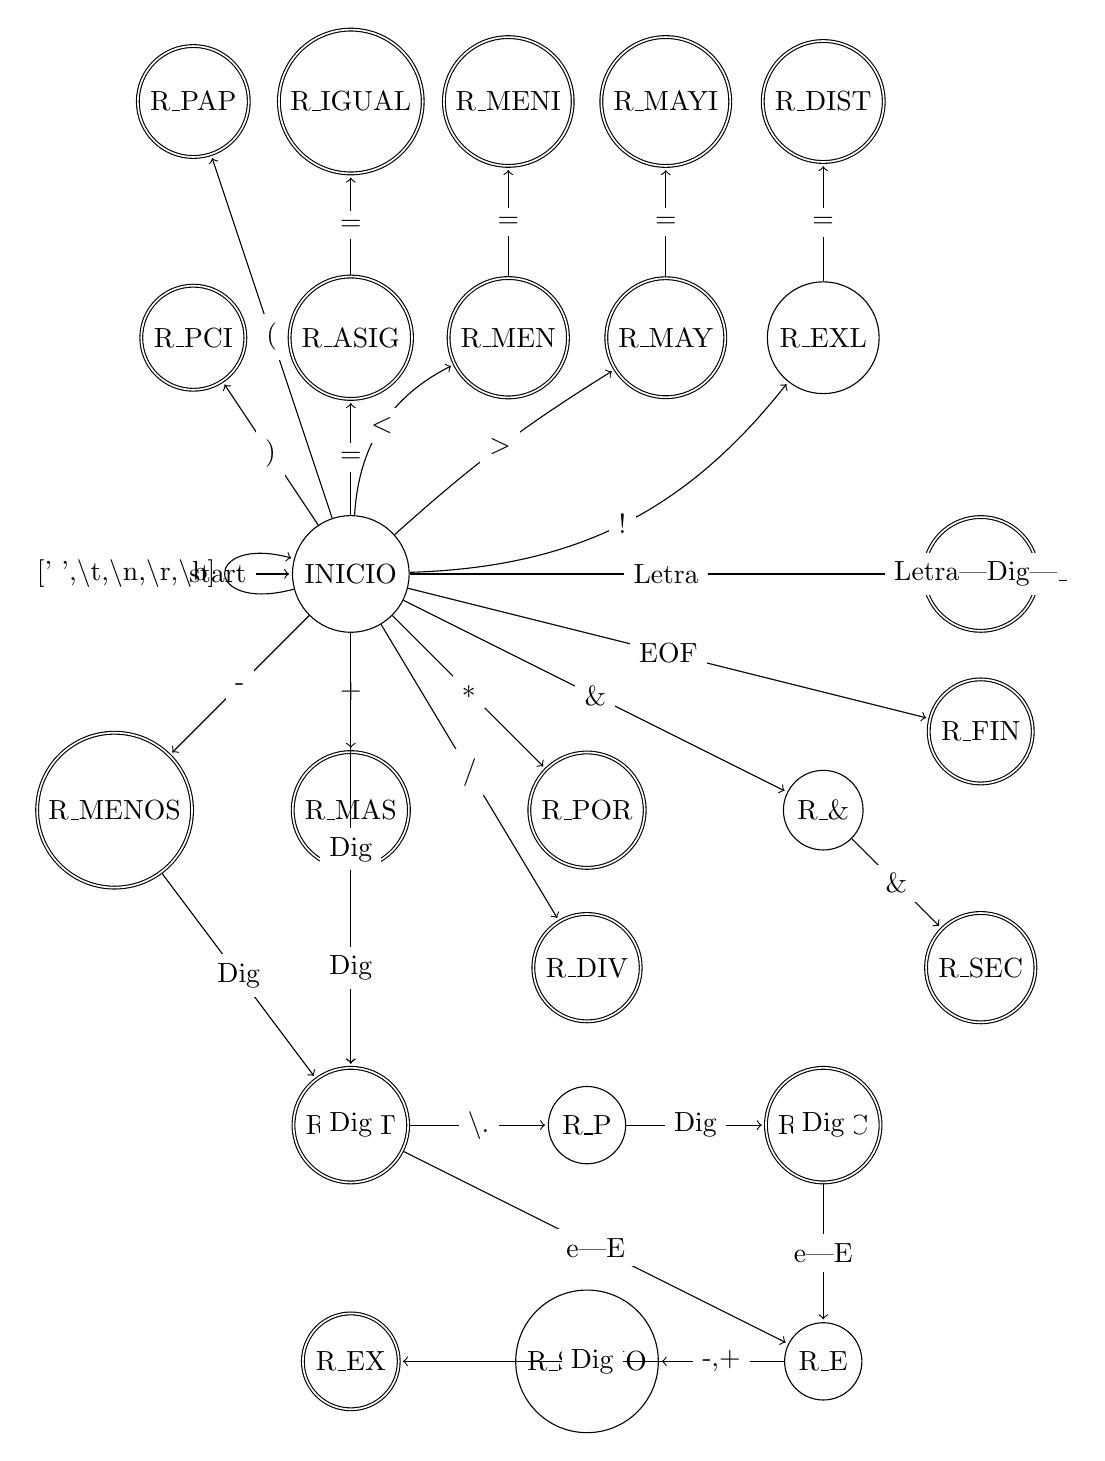
\begin{tikzpicture}[shorten >=1pt,node distance=2cm,on grid,auto]
    \node[state,initial] (q_0) {INICIO};
    \node[state, accepting] (q_1) [above=3of q_0]  {R\_ASIG};
    \node[state, accepting] (q_2) [left=2of q_1] {R\_PCI};
    \node[state, accepting] (q_3) [above=3of q_2] {R\_PAP};
    \node[state, accepting] (q_4) [above=3of q_1] {R\_IGUAL};
    \node[state, accepting] (q_5) [right=2of q_1] {R\_MEN};
    \node[state, accepting] (q_6) [right=2of q_5] {R\_MAY};
    \node[state] (q_7) [right=2of q_6] {R\_EXL};
    \node[state, accepting] (q_8) [above=3of q_5] {R\_MENI};
    \node[state, accepting] (q_9) [above=3of q_6] {R\_MAYI};
    \node[state, accepting] (q_10) [above=3of q_7] {R\_DIST};
    \node[state, accepting] (q_11) [below=3of q_0] {R\_MAS};
		\node[state, accepting] (q_12) [left=3of q_11] {R\_MENOS};
    \node[state, accepting] (q_13) [right=3of q_11] {R\_POR};
    \node[state, accepting] (q_14) [below=of q_13] {R\_DIV};
    \node[state, accepting] (q_15) [below=4of q_11] {R\_ENT};
    \node[state] (q_16) [right=3of q_15] {R\_P};
    \node[state, accepting] (q_17) [right=3of q_16] {R\_DEC};
    \node[state] (q_18) [below=3of q_17] {R\_E};
    \node[state] (q_19) [left=3of q_18] {R\_SIGNO};
    \node[state, accepting] (q_20) [left=3of q_19] {R\_EX};
    \node[state, accepting] (q_21) [right=8of q_0] {R\_VAR};
    \node[state, accepting] (q_22) [below=2of q_21] {R\_FIN};
    \node[state] (q_23) [below=6of q_7] {R\_\&};
    \node[state, accepting] (q_24) [below=3of q_22] {R\_SEC};
			\path[->]
          (q_0) edge [loop left] node {$[$' ',\textbackslash t,\textbackslash n,\textbackslash r,\textbackslash b]} (q_0)
                edge node [fill=white, anchor=center, pos=0.5]          {=} (q_1)
                edge node [fill=white, anchor=center, pos=0.5]     {$)$} (q_2)
                edge node [fill=white, anchor=center, pos=0.5]           {$($} (q_3)
                edge [bend left]        node [fill=white, anchor=center, pos=0.5]           {$<$} (q_5)
                edge [bend left=5] node [fill=white, anchor=center, pos=0.5] {$>$} (q_6)
                edge [bend right=25] node [fill=white, anchor=center, pos=0.5] {!} (q_7)
                edge node [fill=white, anchor=center, pos=0.5] {+} (q_11)
                edge node [fill=white, anchor=center, pos=0.5] {-} (q_12)
                edge node [fill=white, anchor=center, pos=0.5] {$\ast$} (q_13)
                edge  node [fill=white, anchor=center, pos=0.5] {/} (q_14)
                edge  node [fill=white, anchor=center, pos=0.5] {Dig} (q_15)
                edge  node [fill=white, anchor=center, pos=0.5] {Letra} (q_21)
                edge  node [fill=white, anchor=center, pos=0.5] {EOF} (q_22)
                edge  node [fill=white, anchor=center, pos=0.5] {\&} (q_23)
          (q_1) edge  node[fill=white, anchor=center, pos=0.5]     {=} (q_4)
          (q_5) edge  node [fill=white, anchor=center, pos=0.5]            {=} (q_8)
          (q_6) edge  node [fill=white, anchor=center, pos=0.5]            {=} (q_9)
          (q_7) edge node [fill=white, anchor=center, pos=0.5] {=} (q_10)
          (q_11) edge node [fill=white, anchor=center, pos=0.5] {Dig} (q_15)
          (q_12) edge node [fill=white, anchor=center, pos=0.5] {Dig} (q_15)
          (q_15) edge node [fill=white, anchor=center, pos=0.5] {Dig} (q_15)
                 edge node [fill=white, anchor=center, pos=0.5] {\textbackslash .} (q_16)
                 edge node [fill=white, anchor=center, pos=0.5] {e|E} (q_18)
          (q_16) edge node [fill=white, anchor=center, pos=0.5] {Dig} (q_17)
          (q_17) edge node [fill=white, anchor=center, pos=0.5] {Dig} (q_17)
                 edge node [fill=white, anchor=center, pos=0.5] {e|E} (q_18)
          (q_18) edge node [fill=white, anchor=center, pos=0.5] {Dig} (q_20)
                 edge node [fill=white, anchor=center, pos=0.5] {-,+} (q_19)
          (q_21) edge node [fill=white, anchor=center, pos=0.5] {Letra|Dig|\_} (q_21)
          (q_23) edge node [fill=white, anchor=center, pos=0.5] {\&} (q_24);
  \end{tikzpicture}
	
\end{document}


